\documentclass[UTF8]{ctexart}
\pagestyle{plain}
\usepackage{amsmath}
\usepackage{amsfonts}
\usepackage{geometry}
\geometry{a4paper,scale=0.8}
\usepackage{enumitem}
\setlist[description]{leftmargin=\parindent,labelindent=\parindent}
\usepackage{graphicx}
\usepackage{float}
\usepackage{subfigure}
\title{文本分类算法综述}
\author{罗伟斌}
\begin{document}
\maketitle
\section{简介}
	在当今信息爆炸的世界,我们可以接触到海量各种各样的数据和信息,包括文本、声音、图像等,而在这海量信息中大部分的都是以文本方式存在的,比如,电子文档,电子邮件等。海量的信息同样也带来了信息杂乱的烦恼,为了快速、准确地找到我们所需要的信息,我们就必须对这些文本进行有效的管理和组织,挖掘蕴藏在其中的文本信息。文本分类技术作为一个能有效管理和发掘文本信息的技术,在过去的几十年中得到了蓬勃的发展,并且已经在信息检索、医疗诊断、新闻分类、搜索引擎等众多领域得到了广泛的应用。

\subsection{文本分类问题定义}
	\par 文本分类问题可以定义为如下:将布尔值(Boolean)赋予属于集合$D×C$中的每一对记录$<d_j , c_i>$,D表示文本的集合,$C=\{c_1 , c_2 , c_3 ,\ldots , c_{|C|}\}$是预定义类标签值的集合。若项$<d_j, c_i>$被赋予布尔值T则表示文本$d_j$的类标签为$c_i$, 若项$<d_j,c_i>$被赋予布尔值为F,则代表文本$d_j$的类标签不为$c_i$。简而言之,文本分类任务就是找出未知函数$\tilde{\Phi}:D×C\to\{T,F\}$,使得$\tilde{\Phi}$尽可能的近似于或接近于目标函数函数$\Phi$,$\tilde{\Phi}$被称为分类器,也叫假设或者模型。我们假定在文本分类任务中已满足如下条件,类标签值为符号值,并不包含额外含义。除了文本本身内容之外,不包含文本类型,发布日期等外在信息。

\subsection{单标签与多标签文本分类}
	\par 在不同的应用场景中,可能会对文本分类任务加入额外的约束条件,比如限定对于$d_j\in D$只能有确定的K个标签值,其中当K为1时,被称之为单标签分类(single-label classification), 对于每个$d_j\in D$, K可以为0到$|C|$时,称之为多标签分类(multilabel classification)。单标签分类中有个特殊情况是二分类,则意味着$d_j\in D$要么标签值为ci要么为$\overline{c_i}$。
	\par 多标签分类问题可以转化为多个二分类问题,只需要将在标签集合$C=\{c_1,\ldots, c_{|C|}\}$下的多标签分类分解为$\vert C \vert$个独立的在标签集合$\{c_i, \tilde{c_i} \}$(i=1, ......, $\vert C \vert$)二分类问题。当然上面的转换必须保证上述标签集中必须是统计意义上两两相互独立的,对于任意的$c'$, $c''$, $\tilde{\Phi}(d_j, c')$
	与$\tilde{\Phi}(d_j, c')$相互独立。这也就意味着当符合上述条件时,对于单标签文本分类问题的算法可以使用与多标签文本分类问题,但是反过来一般是不成立的。

\subsection{文本分类的应用与方法}
    \par 文本分类技术已经在文本挖掘的多个领域得到了广泛的应用,以下介绍几个最典型的应用场景:
    \begin{description}
    	\item[新闻分类与管理] 现今新闻机构每天都会产生大量的新闻稿件,以至于新闻服务机构(如新闻门户网站)通过无法通过人工有效管理和分门别类,因此文本分类技术在新闻分类方面被广泛应用也就不足为奇了。 
    	\item[文档管理与查询] 除了新闻服务机构,需要处理大量文本文档的地方都有文本分类技术的用武之地,比如在大型的电子图书馆,互联网存档机构和科技著作管理机构等这些地方,对文档良好的层次化管理对查询效率有很大的帮助。
    	\item[情感分析] 微博,论坛,购物网站等等类似的网站都会有大量的用户数据生成,对用户或顾客的反馈或评价进行整理和分析,了解用户的观点,态度,情感倾向等,可以得有用的具有指导性信息。
    	\item[垃圾邮件检测] 像Google或微软等公司都在其邮箱应用中使用文本分类技术来加强对垃圾邮件的过滤,以便向用户提供更好的服务。
    \end{description}
	\par 由于文本分类本身是一个分类问题,因此一般的模式分类方法都可以应用于文本分类的研究。但是在介绍这些算法之前,首先应该了解的如何获取各种文本特征,各种特征应该赋予多大的权值,已经有多种可以表征文本特征的方法,这其中包括了基于文档频率(document frequency)的特征提取,基尼系数(gini-index),信息增益(information gain),$\chi^2$统计量和互信息(mutual information)等方法。通过这些方法可以获得文本的多方面特征,有了这些特征,可以将文本表示成空间向量形式(vector space),近年来的研究是以词嵌入(word embedding)来表征词,进而构建对文本的表示形式。对不同表示形式的文本一般需要设计不同的处理方法。主要的文本分类方法有:
	\begin{description}
		\item[朴素贝叶斯分类器]贝叶斯分类首先假设文本特征之间是相互独立的,然后学习特征与类标签之间的联合概率分布。贝叶斯分类由于其实现非常简单,效率很高,在某些场景下很常用。
		\item[决策树]决策树是一种对实例进行分类的树形结构,可以认为是if-then的规则的集合,也可以认为是定义在特征空间与类空间上的条件概率分布。用决策树进行分类,首先对文本的某一特征进行测试,根据测试结果,将实例分配到不同的子节点,每个子节点对应特征的一个取值,然后递归测试并分配实例,直到分类完成。
		\item[SVM分类]SVM分类是在特征空间上以最大间隔为条件,尝试进行分类的线性或非线性分类器。应用在文本分类中,关键之处在于确定类标签之间的最佳边界。
		\item[kNN最近邻法] kNN最近邻算法是对一个给定文本,在训练数据集中查找离它最近的k个临近文本,根据这些临近文本的分类来给该文本的候选类别评分,最终给出该文本的类别或标签。
		\item[线性最小平方拟合] 线性最小平方拟合方法目的是找到一种从词、短语等构成文本的基本要素到类别标签之间的一种映射关系。
		\item[神经网络分类]将神经网络应用于文本分类的研究越来越多,在某些方面取得了超越之前研究的成绩,卷积神经网络,循环神经网络以及注意力机制都已经被用于文本分类任务上。
	\end{description}
	\par 接下来内容首先将会简要介绍上述前六种文本分类的算法,然后着重聚焦于神经网络分类的方法。
	
\section{分类器的设计}

\subsection{朴素贝叶斯分类器}	
	朴素贝叶斯分类器的基本思想是利用特征项和类别的联合概率分布来估计给定文档的类别概率。假设文本是基于词的一元模型,即文本中的当前词的出现依赖于文本的类别,但是不依赖于其他词及文本的长度,也就是说,词与词之间是独立的。根据贝叶斯公式,文档$d$属于类别$c_i$的概率为\begin{displaymath}P(c_i \vert d)=\frac{P(c_i \vert d)\times P(c_i)}{P(d)} \end{displaymath}
	\par 在具体实现时,有两种具体情况:
	\begin{enumerate}
		\item 文档$d_j$采用DF向量表示法,即文档向量V的分量为一个布尔值,0表示相应的特征向量在该文档未中出现,1表示特征在文档中出现。这时
		\begin{eqnarray}
			\nonumber P(d \vert c_i)=\prod_{t_j\in V} P(d(t_j) \vert c_i)  \\ 
			\nonumber P(d)=\sum_i[P(c_i)\prod_{t_j\in V} P(d(t_j) \vert c_i)]
		\end{eqnarray}
	因此,
		\begin{displaymath}
			P(c_i \vert d)=\frac{P(c_i)\prod_{t_j\in V} P(d(t_j) \vert c_i)}{\sum_i[P(c_i)\prod_{t_j\in V} P(d(t_j) \vert c_i)]}
		\end{displaymath}
	其中,P($c_i$)为$c_i$类文档的概率,P(d($t_j$) $\vert$ $c_i$)是对$c_i$类文档中特征$t_j$出现的条件概率的拉普拉斯估计。
		\item 若文档d采用的是TF向量表示法,即文档向量V的分量为相应的特征在该文档中的出现频度,这文档d属于$c_i$类的概率为
		\begin{displaymath}
			P(c_i \vert d)=\frac{P(c_i)\prod_{t_j\in V} P(t_j \vert c_i)^{TF(t_j, d)}}{\sum_i[P(c_i)\prod_{t_j\in V} P(t_i \vert c_i)^{TF(t_j, d)}]}	
		\end{displaymath}
	其中,TF($t_j$,d)是文档d中特征$t_j$出现的频度,P($t_i \vert c_i$)是对$c_i$类文档中特征$t_i$出现的条件概率的拉普拉斯估计。
	\end{enumerate}

\subsection{决策树分类器}
	决策树分类器其出发点是:大量复杂的系统组成普遍存在分层现象,或者说复杂任务是可以通过层次化分解完成的,文本分类过程也类似。
	\par 决策树是一棵树,树的根节点是整个数据集合空间,每个分节点是对一个单一特征的测试,该测试将数据集合空间分割成两个或更多个类别,即决策树可以是二叉树也可以是多叉树。每个叶节点是属于单一类别的记录。构造决策树分类器时,首先要通过训练生成决策树,然后再通过测试集对决策树进行修剪。一般可以通过递归分割的过程构建决策树,其生成的过程通常是自上而下的,选择分割的方法有多种,但是目标都是一致的,就是对目标文档进行最佳分割。从根节点到叶节点都有一条路径,这条路径就是一条决策“规则”。\par 决定那个特征作为目前的最佳分类特征时,一般的做法时穷尽所有的特征,对每个特征分裂的好坏进行量化,从而计算出最佳分裂。信息增益时决策树训练中常用的衡量给定特征区分训练数据样本能力的定量标准。在决策树的训练过程中,信息增益等价于训练数据集中类与特征的互信息,可用如下公式计算:
	\begin{displaymath}
		g(D,A)=H(D)-H(D \vert A)
	\end{displaymath}
	其中,g(D,A)表示特征A对训练数据集D的信息增益,H(D)为集合D的经验熵,H(D$\vert$A)表示特征A给定条件下D的经验条件熵。

\subsection{SVM分类器}
	基于支持SVM的分类方法主要用于解决二元模式分类问题,其出发点是在向量空间中找到一个决策平面,这个平面能“最好”的分割两个分类中的数据点。SVM分类法就是要在训练集中找到具有最大类间界限的决策平面。\par 由于SVM算法是基于二分类的,因此对于对类别分类问题通常需要建立多个二类分类器。与线性判别函数一样,它的结果强烈地依赖于已知数据集的构造。对于非线性问题可以采用核技巧进行映射。
	\par 对于线性可分情况:设训练集为$T=\{(x_1,y_1),\ldots \},(x_1,y_1)\in (X \times Y)$,其中X=$R_n$,Y=\{-1,1\}。线性可分表明存在这规范超平面,可以将训练数据中的正负两类分别位于超平面的两侧,且集合间隔为2/$\Vert$ $\omega$ $\Vert$,从而得到原始问题的最优化问题:
	\begin{align*}
		&\min_{\omega,b} \frac{1}{2}{\Vert \omega \Vert} \\
		&s.t\quad y_i(\omega{x_i}+b)-1\ge 0
	\end{align*}
	由此可以得到分类超平面:
	\begin{displaymath}
		\omega^* \cdot x + b^* = 0
	\end{displaymath}
	分类决策函数为:
	\begin{displaymath}
		f(x)=sign(\omega^* \cdot x + b^*)
	\end{displaymath}

\subsection{kNN最近邻法}
	kNN最近邻法将在训练集中查找离测试文档最近的k个邻近文档,把邻近文档和测试文档的相似度作为邻近文档所在类别的权重,如果这k个邻近文档中的部分文档属于同一个类别,则将该类别中每个邻近文档的权重求和,并作为该类别和测试文档的相似度。然后,通过对候选分类评分的排序,给出一个阈值。决策规则可以写作:
	\begin{displaymath}
		y(x,c_j)=\sum_{d_i\in kNN}sim(x,d_i)y(d_i,c_j)-b_j
	\end{displaymath}
	其中,$y(d_i,c_j)$取值为0或1,取值为1表示文档$d_i$属于类别$c_j$,取值为0时表示文档$d_i$不属于分类$C_j$;$sim(x,d_i)$表示测试文档x和训练文档$d_i$之间的相似度;$b_j$是二元决策的阈值。一般地,采取两个向量夹角的余弦值来度量向量之间的相似度。

\subsection{线性最小平方拟合法}
	线性最小平方拟合是一种映射方法,其出发点是从训练集和分类文档中学习得到多元回归模型。其中训练数据用输入/输出向量表示,输入向量是用传统向量空间模型表示的文档(词和对应的权重),输出向量则是文档对应的分类(带有0-1权重)。通过在向量的训练对上求解线性最小平方拟合,得到一个“词-分类”的回归系数矩阵:
	\begin{displaymath}
		F_{LS}=arg\min {\Vert F \times A - B \Vert}^2
	\end{displaymath}
	其中,矩阵A和矩阵B描述的是训练数据(对应栏分别是输入和输出向量);$F_{LS}$为结果矩阵,定义了从任意文档到加权分类向量的映射。对这些分类的权重映射值排序,同时结合阈值算法,就可以来判别输入文档所属的类别。阈值是从训练中学习获取的。

\section{基于神经网络的文本分类方法}
	深度学习是机器学习的一个分支,是神经网络的重命名。神经网络是一系列学习技术,受到模拟脑工作计算的启发,可以被看作是学习可微的数学函数。
	\par 虽然与上一小节介绍的算法同属机器学习算法,都是基于过去的观测(数据)学习如何做出预测,但是神经网络学习方法不仅学习预测,而且学习正确地表示数据,以便获得更好的预测结果。给出一个足够大的训练数据集(输入与输出的映射集合),然后将数据“喂”给一个神经网络,其产生的输入的后继转换,直到用最终的转换来预测输出。神经网络产生的转换都学习自给定的数据(输入输出映射),以便每个转换都使得更易于将数据和期望的标签之间建立联系。
	\par 设计基于神经网络的分类器,我们将主要聚焦于设计合理的网络结构和训练方式,提供给网络合适的输入输出训练数据实例集合,将输入数据恰当的编码表示,神经网络将自动地执行大量的学习工作。
	\par 本小节首先介绍神经网络基本知识和构造适合神经网络的文本特征的方法,然后将详细介绍几种应用于文本分类任务的神经网络结构。

\subsection{前馈神经网络}
	神经网络的灵感来源于大脑的计算机制,它由被称为神经元的单元组成。虽然人工神经网络与大脑之间的联系实际上相当的薄弱,但是这个比喻确一直沿用了下来。最简单的神经网络如下图所示,这个神经网络仅由一个“神经元”构成。
	\begin{figure}[H]
		\centering 
		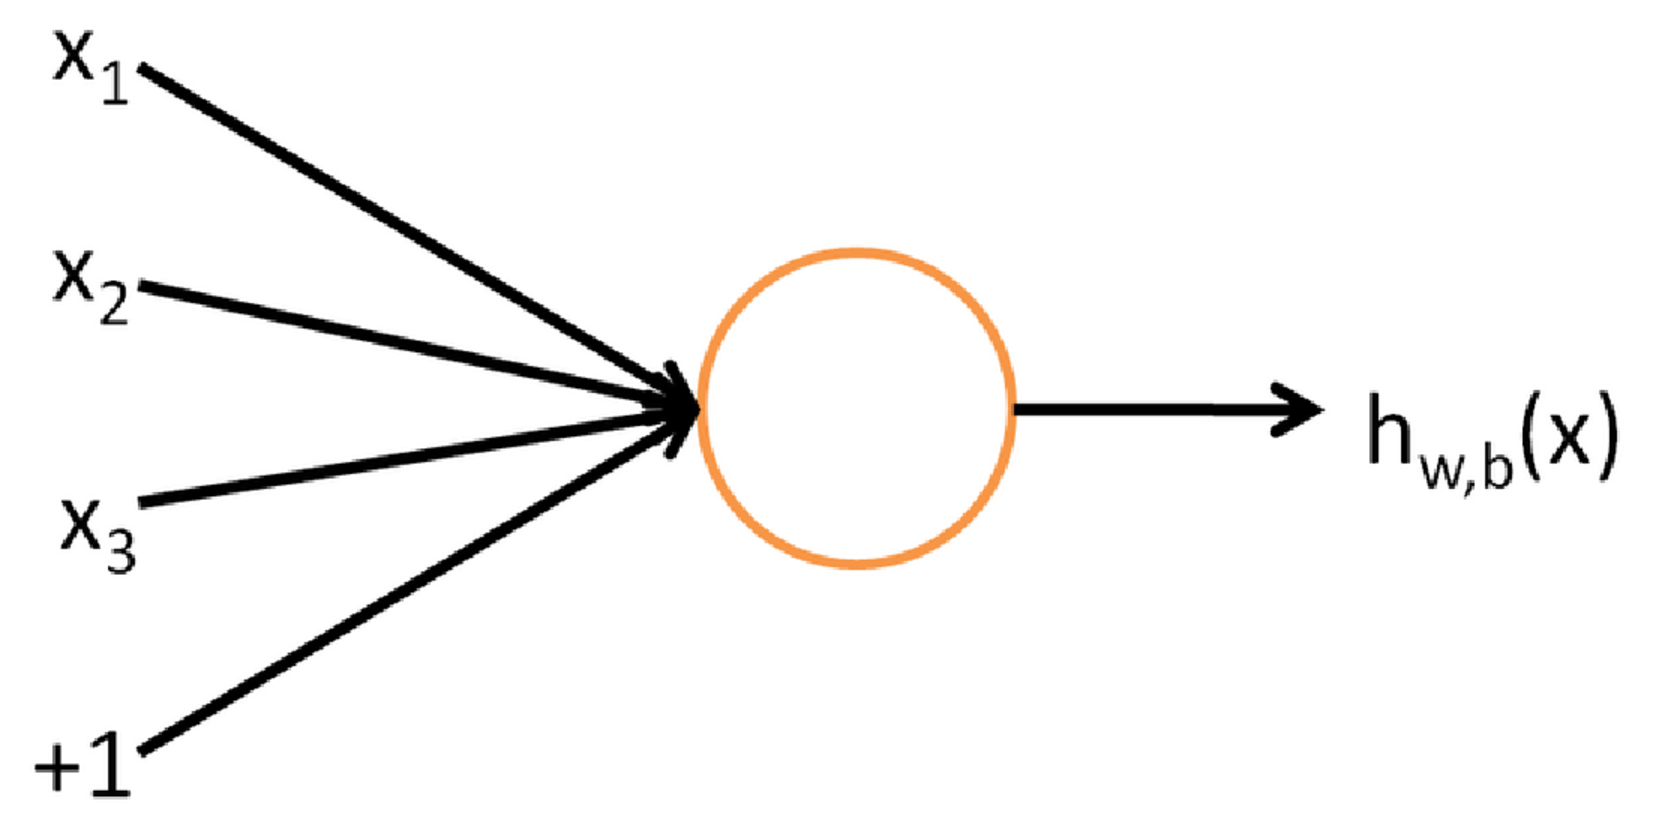
\includegraphics[width=0.5\textwidth]{SingleNeuron}
	\end{figure}
	这个“神经元”是一个以$x_1, x_2, x_3$及截距+1 为输入值的运算单元,其输出为 $h_{W,b}(x) = f(W^Tx) = f(\sum_{i=1}^3 W_{i}x_i +b)$ ,其中函数$f : \Re \mapsto \Re$ 被称为“激活函数”。
	神经网络就是将许多个单一“神经元”联结在一起,这样,一个“神经元”的输出就可以是另一个“神经元”的输入。下图是一个三层神经网络。
	\begin{figure}[H]
		\centering
		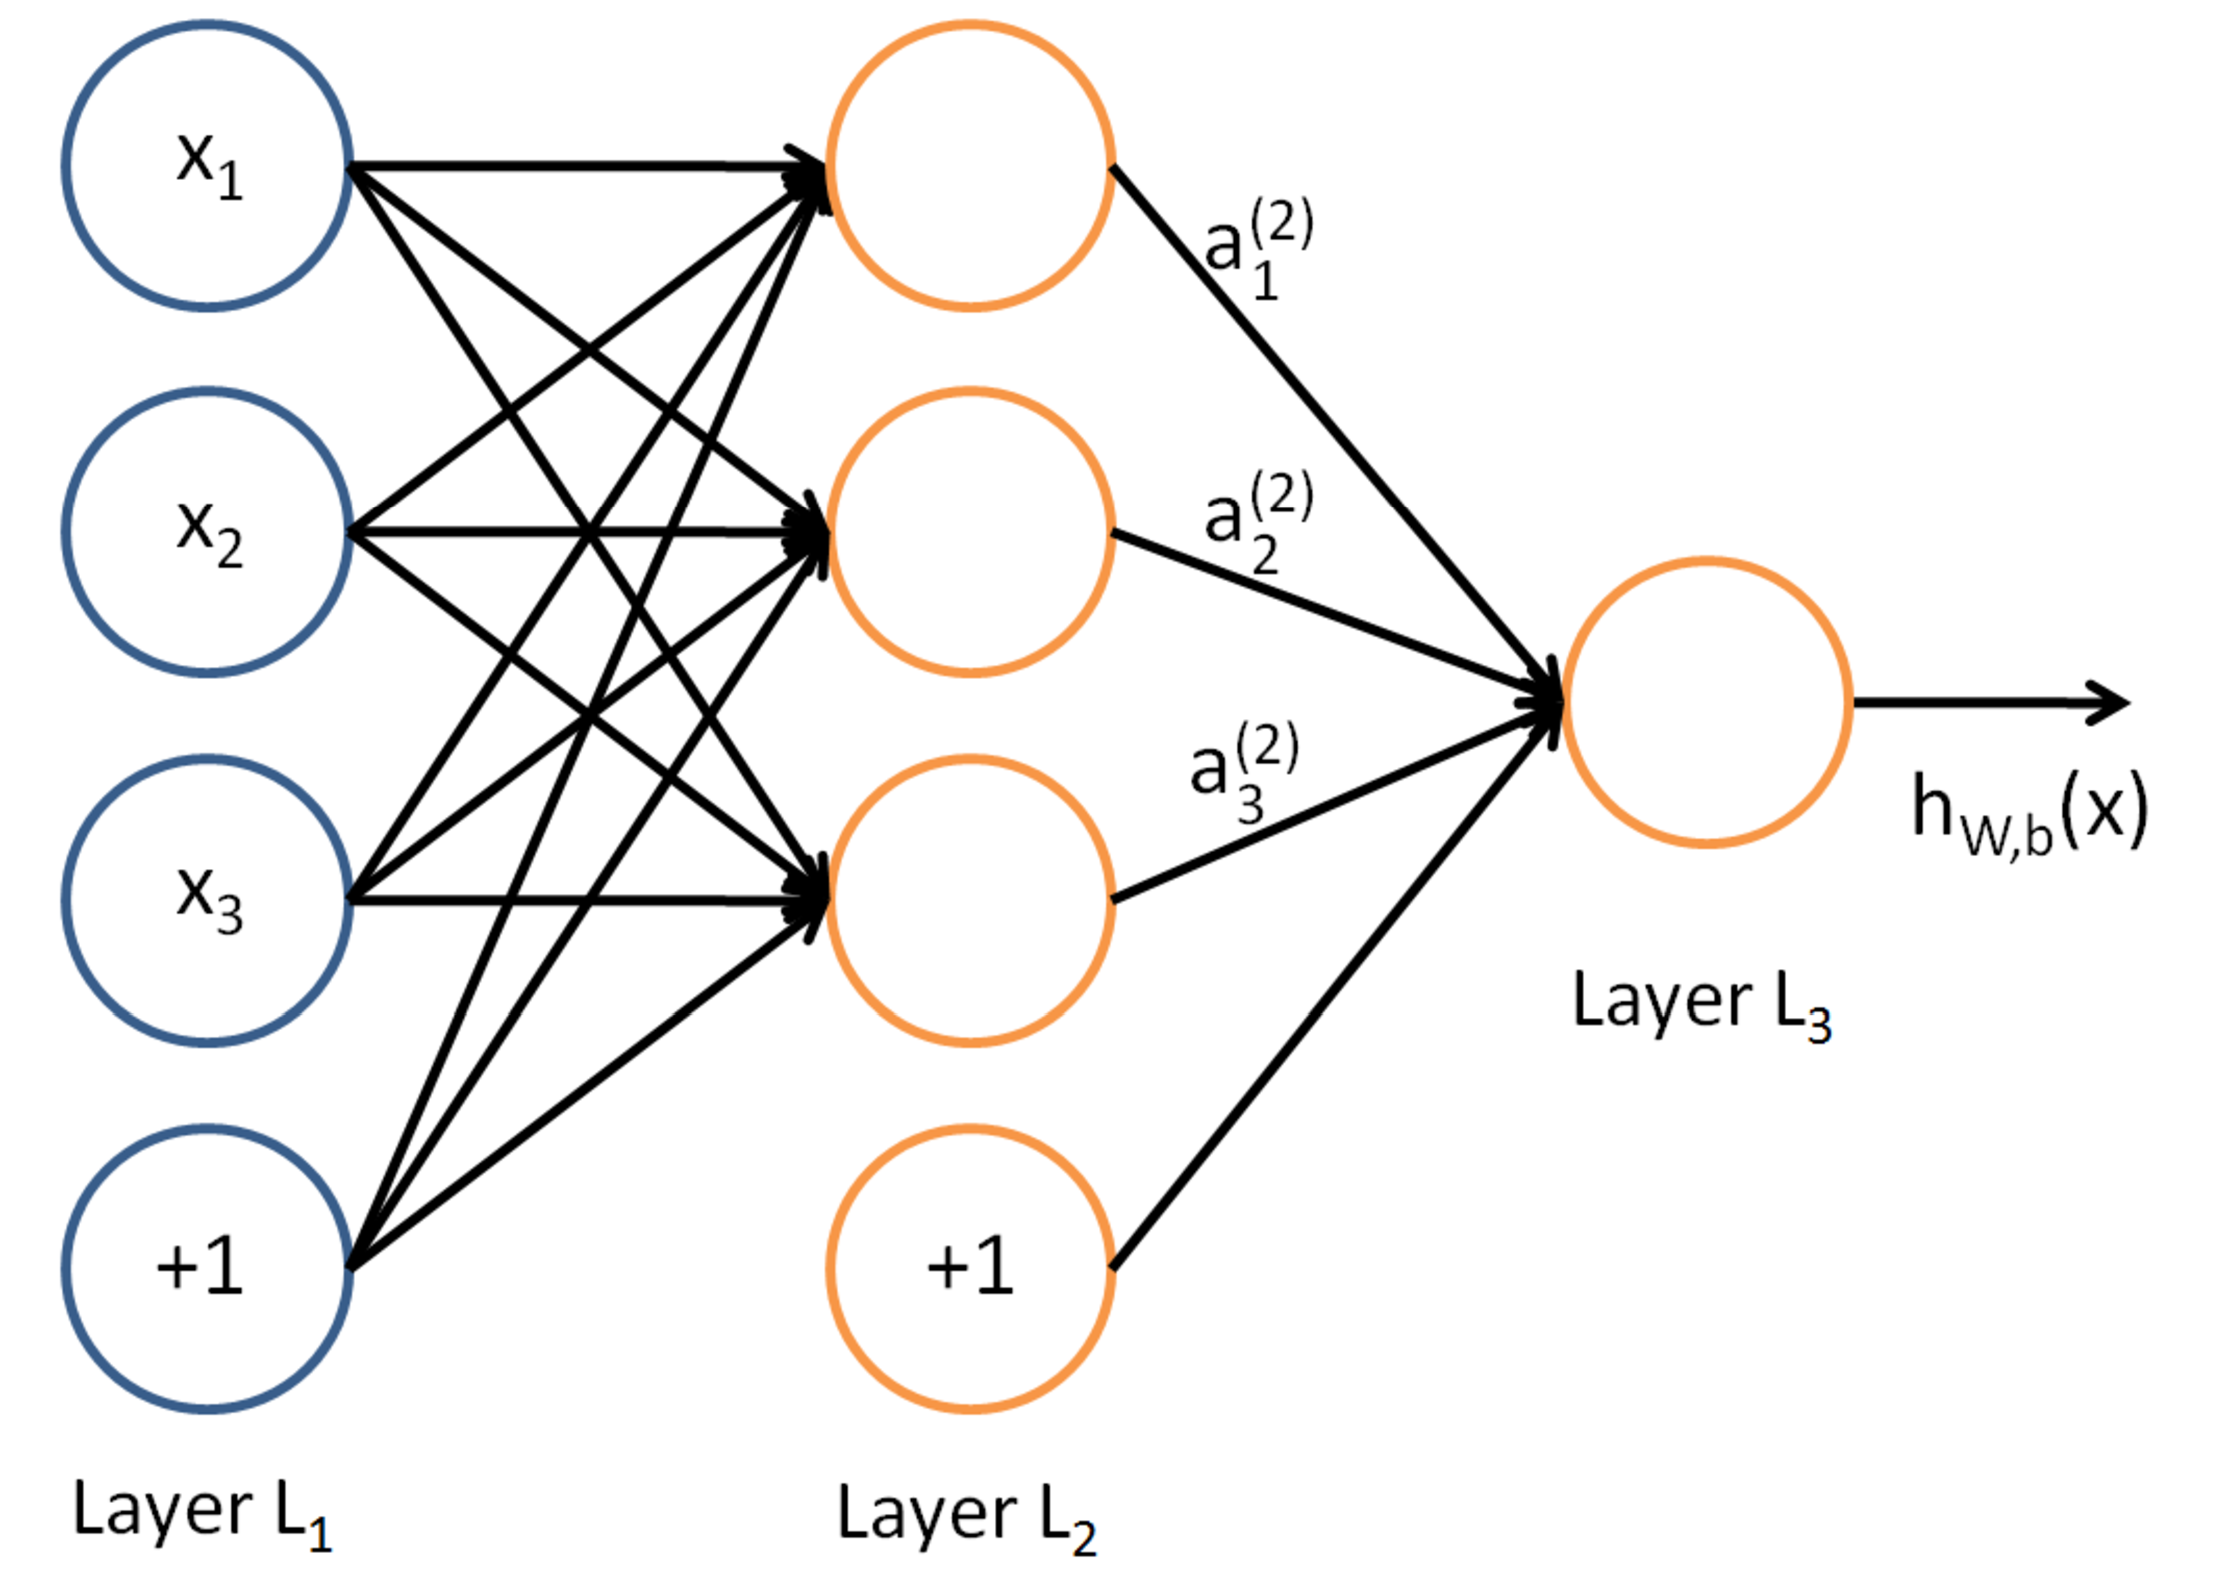
\includegraphics[width=0.5\textwidth]{Network331}
	\end{figure}
	圆圈表示神经网络的输入,标上“+1”的圆圈被称为偏置节点,也就是截距项。神经网络最左边的一层叫做输入层,最右的一层叫做输出层(本例中,输出层只有一个节点)。中间所有节点组成的一层叫做隐藏层,因为不能在训练样本集中观测到它们的值。$n_l$来表示网络的层数,将第l层记为$L_l$ ,于是$L_1$是输入层,输出层是$L_{n_l}$。上图神经网络有参数$(W,b) = (W^{(1)}, b^{(1)}, W^{(2)},b^{(2)})$,其中$W^{(l)}_{ij}$(下面的式子中用到)是第l层第j单元与第l+1层第i单元之间的联接参数(其实就是连接线上的权重,注意标号顺序),$b^{(l)}_i$是第l+1层第i单元的偏置项。同时,我们用$s_l$ 表示第l层的节点数(偏置单元不计在内)。$a^{(l)}_i$ 表示第l层第i单元的激活值(输出值)。当l=1 时,$a^{(1)}_i = x_i$,也就是第i个输入值(输入值的第i个特征)。	用$z^{(l)}_i$表示第l层第i单元输入加权和(包括偏置单元),那么给定对于给定参数集合W,b以及第l层的激活值$a^{(l)}$后,第l+1层的激活值$a^{(l+1)}$就可以按照下面步骤计算得到,从而可以求得整个网络激活值,上述计算过程就是前馈神经网络的前向传播。
	\begin{align*} 
		z^{(l+1)} &= W^{(l)} a^{(l)} + b^{(l)} \\ a^{(l+1)} &= f(z^{(l+1)}) 
	\end{align*} 
	比如上图神经网络的计算步骤如下:
	\begin{align*} 
	a_1^{(2)} &= f(W_{11}^{(1)}x_1 + W_{12}^{(1)} x_2 + W_{13}^{(1)} x_3 + b_1^{(1)}) \\ a_2^{(2)} &= f(W_{21}^{(1)}x_1 + W_{22}^{(1)} x_2 + W_{23}^{(1)} x_3 + b_2^{(1)}) \\ a_3^{(2)} &= f(W_{31}^{(1)}x_1 + W_{32}^{(1)} x_2 + W_{33}^{(1)} x_3 + b_3^{(1)}) \\ h_{W,b}(x) &= a_1^{(3)} = f(W_{11}^{(2)}a_1^{(2)} + W_{12}^{(2)} a_2^{(2)} + W_{13}^{(2)} a_3^{(2)} + b_1^{(2)}) 
	\end{align*} 
	
\subsection{反向传播算法}
求解神经网络可以用梯度下降法,其中关键步骤是计算偏导数,而反向传播算法是计算偏导数的一种有效方法。
\par 假设有固定样本集$\{ (x^{(1)}, y^{(1)}), \ldots, (x^{(m)}, y^{(m)}) \}$,它包含m个样例。对于单个样例(x,y),其代价函数为:
\begin{align*} J(W,b; x,y) = \frac{1}{2} \left\| h_{W,b}(x) - y \right\|^2. \end{align*}
给定一个包含m个样例的数据集,我们可以定义整体代价函数为:
\begin{align*} 
	J(W,b) &= \left[ \frac{1}{m} \sum_{i=1}^m J(W,b;x^{(i)},y^{(i)}) \right] + \frac{\lambda}{2} \sum_{l=1}^{n_l-1} \; \sum_{i=1}^{s_l} \; \sum_{j=1}^{s_{l+1}} \left( W^{(l)}_{ji} \right)^2 \\ &= \left[ \frac{1}{m} \sum_{i=1}^m \left( \frac{1}{2} \left\| h_{W,b}(x^{(i)}) - y^{(i)} \right\|^2 \right) \right] + \frac{\lambda}{2} \sum_{l=1}^{n_l-1} \; \sum_{i=1}^{s_l} \; \sum_{j=1}^{s_{l+1}} \left( W^{(l)}_{ji} \right)^2
\end{align*} 
以上关于J(W,b)定义中的第一项是一个均方差项。第二项是一个正则化项(也叫权重衰减项),其目的是减小权重的幅度,防止过度拟合。
使用反向传播算法来计$\frac{\partial}{\partial W_{ij}^{(l)}} J(W,b; x, y)$ 和$\frac{\partial}{\partial b_{i}^{(l)}} J(W,b; x, y)$,这两项是单个样例(x,y) 的代价函数J(W,b;x,y) 的偏导数。一旦我们求出该偏导数,就可以推导出整体代价函数J(W,b) 的偏导数:
\begin{align*} 
	\frac{\partial}{\partial W_{ij}^{(l)}} J(W,b) &= \left[ \frac{1}{m} \sum_{i=1}^m \frac{\partial}{\partial W_{ij}^{(l)}} J(W,b; x^{(i)}, y^{(i)}) \right] + \lambda W_{ij}^{(l)} \\ \frac{\partial}{\partial b_{i}^{(l)}} J(W,b) &= \frac{1}{m}\sum_{i=1}^m \frac{\partial}{\partial b_{i}^{(l)}} J(W,b; x^{(i)}, y^{(i)}) 
\end{align*} 
反向传播算法的思路如下:给定一个样例(x,y),我们首先进行“前向传导”运算,计算出网络中所有的激活值,包括$h_{W,b}(x)$的输出值。之后,针对第 l 层的每一个节点i,我们计算出其“残差”$\delta^{(l)}_i$,该残差表明了该节点对最终输出值的残差产生了多少影响。对于最终的输出节点,我们可以直接算出网络产生的激活值与实际值之间的差距,我们将这个差距定义为$\delta^{(n_l)}_i$第$n_l$层表示输出层)。
\par 反向传播算法可表示为以下几个步骤:\begin{enumerate}
	\item 进行前馈传导计算,利用前向传导公式,得到$L_2$, $L_3$, \ldots 直到输出层$L_{n_l}$的激活值。对输出层(第$n_l$层),计算:
	\begin{align*} \delta^{(n_l)} = - (y - a^{(n_l)}) \bullet f'(z^{(n_l)}) \end{align*} 
	\item 对于l = $n_l-1$, $n_l-2$, $n_l-3$, \ldots, 2的各层,计算:
	\begin{align*} \delta^{(l)} = \left((W^{(l)})^T \delta^{(l+1)}\right) \bullet f'(z^{(l)}) \end{align*} 
	\item 计算最终需要的偏导数值:
	\begin{align*} 
	\nabla_{W^{(l)}} J(W,b;x,y) &= \delta ^{(l+1)} (a^{(l)})^T, \\ \nabla_{b^{(l)}} J(W,b;x,y) &= \delta^{(l+1)}. 
	\end{align*}
\end{enumerate}
\par 求出了偏导数,便可以使用梯度下降法进行迭代,进而求解神经网络。

\subsection{文本特征的构造}
	当考虑一个句子、一个段落或者一篇文章的时候,观察到的特征是字符和词在文本中的数量和次序,还可以直接观测到的就是位置,也就是上下文特征,围绕某个词、句子或段落的其他词、句子或段落也可以作为特征,与目标的距离也是特征,一般来说所具有的信息也越丰富。前面提到过的特征提取方法有基于文档频率,基尼系数,信息增益,$\chi^2$统计量和互信息等,这些方法都是将词当做是离散的不相关的符号,为了获得更准确的文本表示,在基于神经网络的文本分类方法中,大都对词和文本使用分布式表示。
	\par 在分布式表示中,每个词与$\mathbb{R}^d$中的向量相关联,之中相对于某些任务的词的“含义”能够被向量的不同维度以及被其他单词的维度所捕获。分布式表示中维度是不可解释的,并且具体维度不一定对应于特定概念。表示的分布性质意味着某一特定方面的意义可以通过许多维度的组合来捕获,并且给定的维度可能有助于捕捉意义的几个方面。获取词的分布式表示已经有多种算法,比如Collobert和Weston提了一种算法,还有Mikolov及其同事提出的Word2Vec算法,下面将介绍广为流行的Word2Vec。
	\par Word2Vec基于神经语言模型,它具有两种不同的上下文表示方法(CBOW和Skip-gram)和两个不同的优化目标(负采样和层次Softmax),其中负采样目标是关键。Word2vec的负采样通过训练网络来从“坏”的词-上下文对中区分出“好”的词-上下文对。考虑正确的词-上下文对集合D,以及不正确的词-上下文对集合$\overline{D}$,算法的目标是估计来自正确的集合D的词-上下文对的概率$P(D=1 \vert \omega, c)$。对于来自D的对,其得分概率应该高,对于来自$\overline{D}$的对,其得分概率应该低。同时需要满足概率约束规定$P(D=1 \vert \omega, c)$=1-$P(D=0 \vert \omega, c)$。可以将概率建模为如下$s(\omega,c)$:
	\begin{displaymath}
		P(D=1 \vert \omega, c)=\frac{1}{1+e^{-s(\omega,c)}}
	\end{displaymath}
	算法的语料库目标是最大化数据$D\cup \overline{D}$的对数似然函数。
	\begin{displaymath}
		L = \sum_{(\omega,c)\in D}logP(D=1 \vert \omega, c) + \sum_{(\omega,c)\in \overline{D}}logP(D=0 \vert \omega, c)
	\end{displaymath}
	正例集D从语料库中生成,负例集可以通过下面步骤生成:对于每个好的词-上下文对($\omega$,c)$\in$D,采样k个词$\omega_{1:k}$,并将($\omega_i$,c)中的每一个作为负例加到$\overline{D}$。
	\par Word2Vec有两种实现方法,两种结构如下图所示:
	\begin{figure}[H]
		\centering
		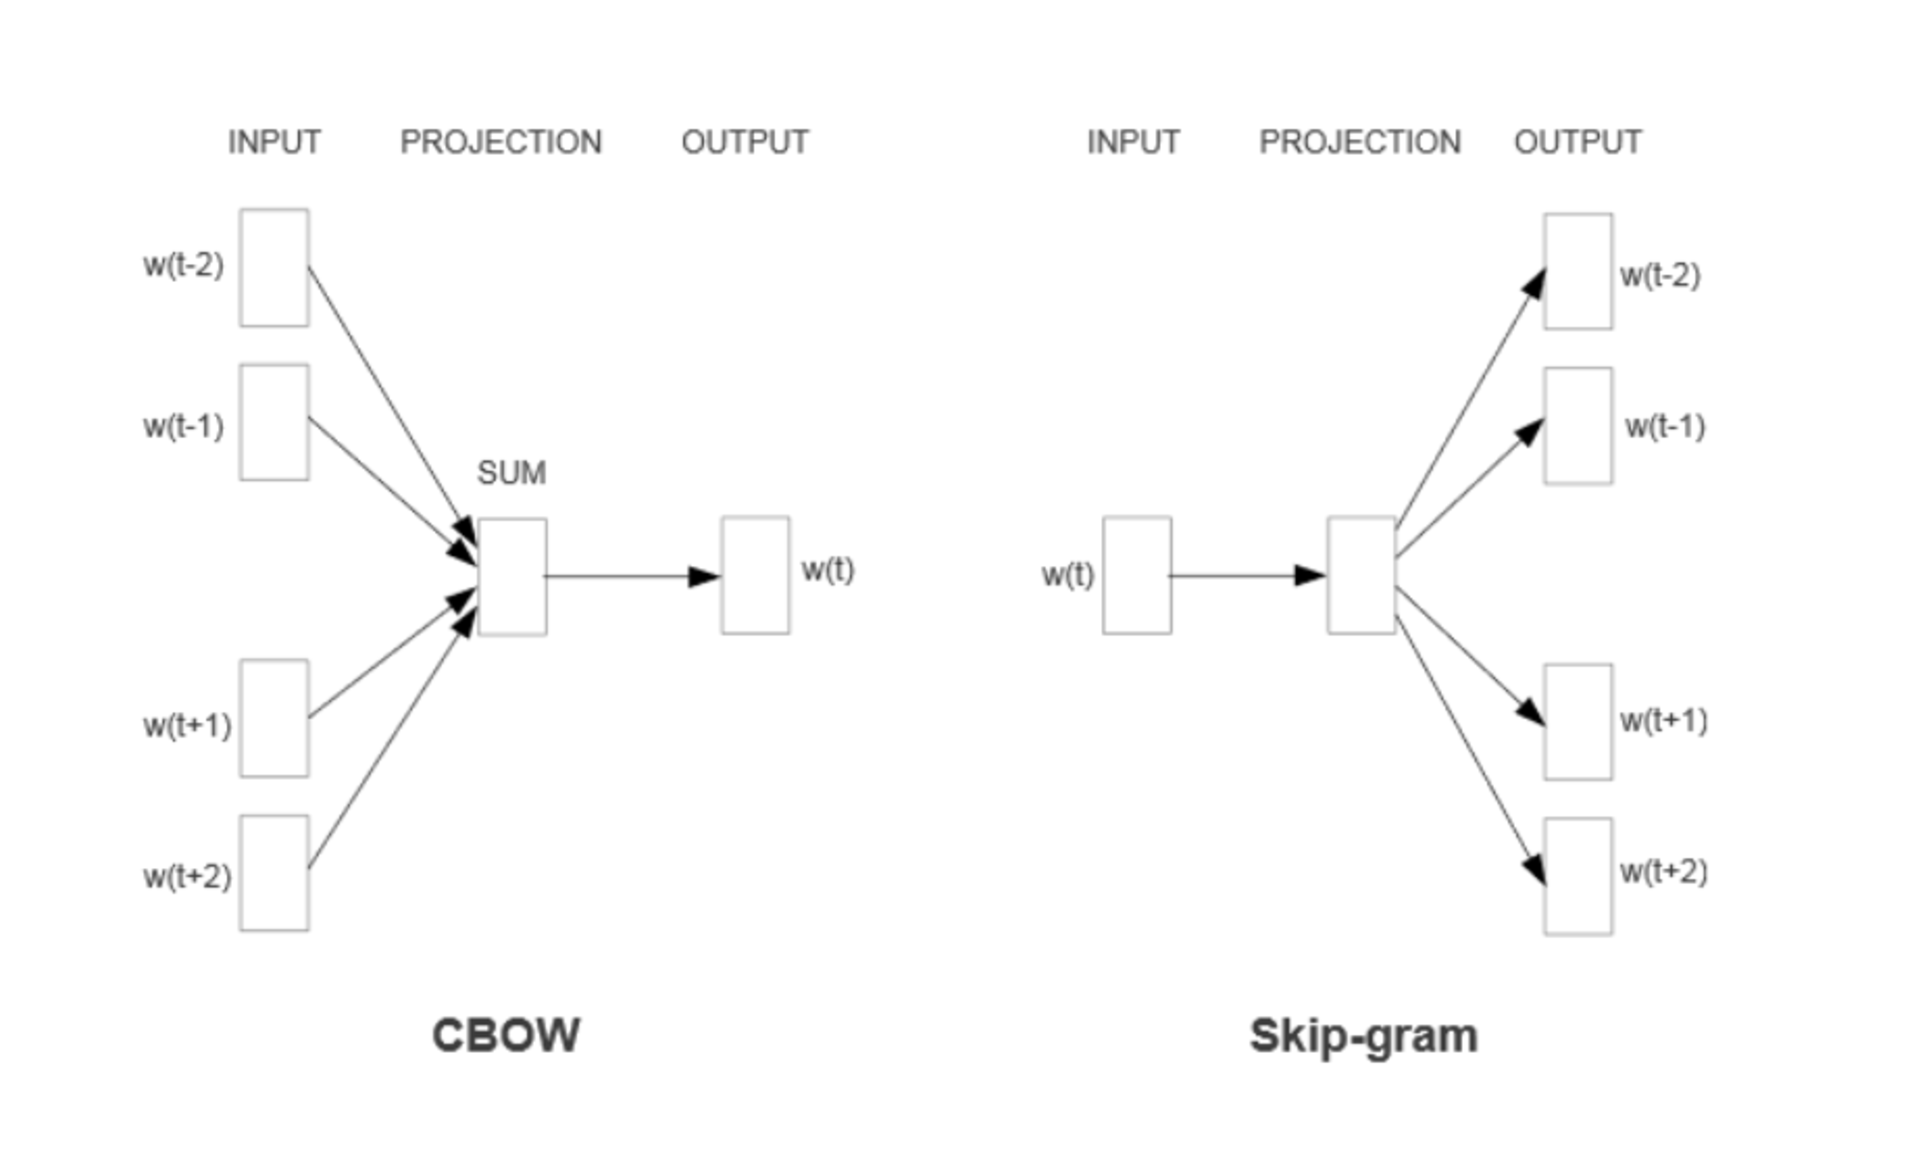
\includegraphics[width=0.5\textheight]{cbow_skip}
	\end{figure}
	\begin{description}
		\item[CBOW] CBOW表示方法将上下文向量c定义为上线问组成的词嵌入向量的累计和:$c = \sum_{i=1}^{k}c_i$。然后将定义得分函数s($\omega$,c)=$\omega$$\cdot$$c$,从而得到:
		\begin{displaymath}
			P(D=1 \vert \omega, c)=\frac{1}{1+e^{-s(\omega \cdot c_1+\omega \cdot c_2+\ldots +\omega \cdot c_k)}}
		\end{displaymath}
		\item[Skip-gram] Skip-gram将上下文中的元素$c_i$和其他元素相独立,即一个词-上下文对($\omega$,$c_{1:k}$)在语料D中表示成k个不同的上下文:($\omega$,$c_{1}$),($\omega$,$c_{2}$),\ldots,($\omega$,$c_{k}$),得分函数于CBOW一样,从而得到:
		\begin{align*}
			&P(D=1 \vert \omega, c_i)=\frac{1}{1+e^{-\omega \cdot c_i}}\\
			&P(D=1 \vert \omega, c_{1:k})=\prod_{i=1}^{k}P(D=1 \vert \omega, c_i)=\prod_{i=1}^{k}\frac{1}{1+e^{-\omega \cdot c_i}}
		\end{align*}
	\end{description}
	\par Word2Vec模型训练带来了两个词向量矩阵,$E^{\omega}\in \mathbb{R}^{\vert v_{\omega} \vert \times d_{emb}}$和$E^{c}\in \mathbb{R}^{\vert v_{c} \vert \times d_{emb}}$分别代表词和上下文的词向量矩阵。可以基于词向量可以用来构造文本的表示,作为神经网络模型的输入。

\subsection{文本分类任务中的神经网络模型}
下面介绍目前在文本分类任务中比较重要的神经网络模型,这些模型大致可以分为三类:基于卷积神经网络的模型,基于循环神经网络的模型,结合卷积神经网络和循环神经网络的模型。

\subsubsection{基于卷积神经网络的模型}
Yoon Kim等人在2014年首先提出了使用卷积神经网络用于文本分类的神经网络模型,整个网络模型架构如下图:
\begin{figure}[H]
	\centering 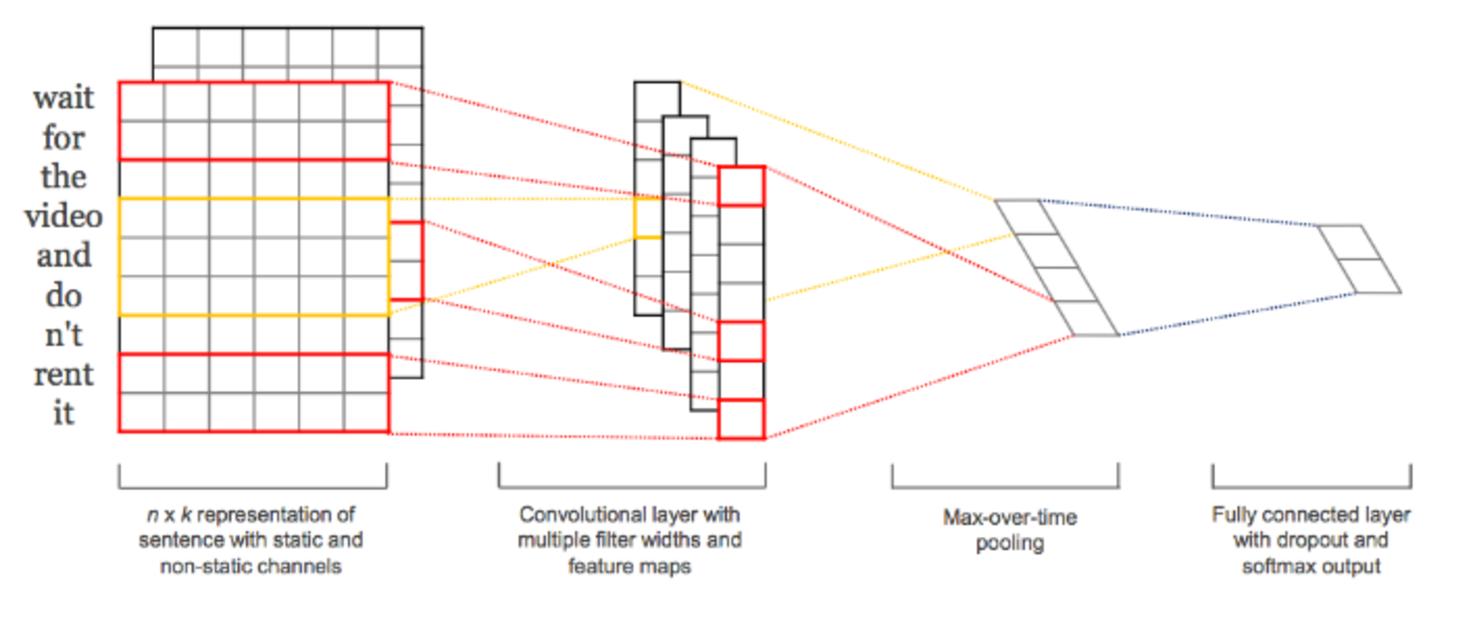
\includegraphics[width=0.5\textheight]{textCNN}
\end{figure}
模型输入是矩阵形式,因此首先是构造矩阵。句子有词构成,使用词向量表示词,再对句子的长度设置一个固定值(可以是最大长度),那么就可以构造一个矩阵,这样就可以应用于这个CNN模型了。整个网络共四层:
\begin{description}
	\item[输入层] 如图所示,输入层是句子中的词语对应的词向量依次(从上到下)排列的矩阵,假设句子有 n 个词,向量的维数为 k ,那么这个矩阵就是 n×k 的。这个矩阵的类型可以是静态的,也可以是动态的。静态就是词向量是固定不变的,而动态则是在模型训练过程中,词向量也当做是可优化的参数。对于未登录词的词向量,可以用0或者随机小的正数来填充。
	\item[卷积层] 输入层通过卷积操作得到若干个Feature Map,卷积窗口的大小为h×k,其中h表示纵向词语的个数,而k表示词向量的维数。通过这样一个大型的卷积窗口,将得到若干个列数为1的Feature Map。
	\item[池化层] 接下来的池化层,采用了Max-over-time Pooling的方法。这种方法就是简单地从之前一维的Feature Map中提出最大的值,最大值代表着最重要的信号。可以看出,这种Pooling方式可以解决可变长度的句子输入问题(因为不管Feature Map中有多少个值,只需要提取其中的最大值)。最终池化层的输出为各个Feature Map的最大值们,即一个一维的向量。
	\item[全连接 + Softmax层] 池化层的一维向量的输出通过全连接的方式,连接一个Softmax层,Softmax层可根据任务的需要设置(通常反映着最终类别上的概率分布)。
\end{description}
	\par Yoon Kim等人提出这个模型很简单,但是却有着很好的性能,并且首次将卷积神经网络的方法引入进来。之后很多研究都是基于Yoon Kim的这个模型。Kalchbrenner等人提出了一种名为DCNN(Dynamic Convolutional Neural Network)的网络模型,采用了Dynamic-pooling的方法来对句子语义进行建模,也取得了不错的效果;Hughes等人在2017年提出了一种应用于临床诊断文本分类的模型也是基于卷积神经网络的,其结构十分类似Yoon Kim提出的模型,不同之处在于其中间有多层卷积层,整体模型结构如下。
	\begin{figure}[H]
		\centering 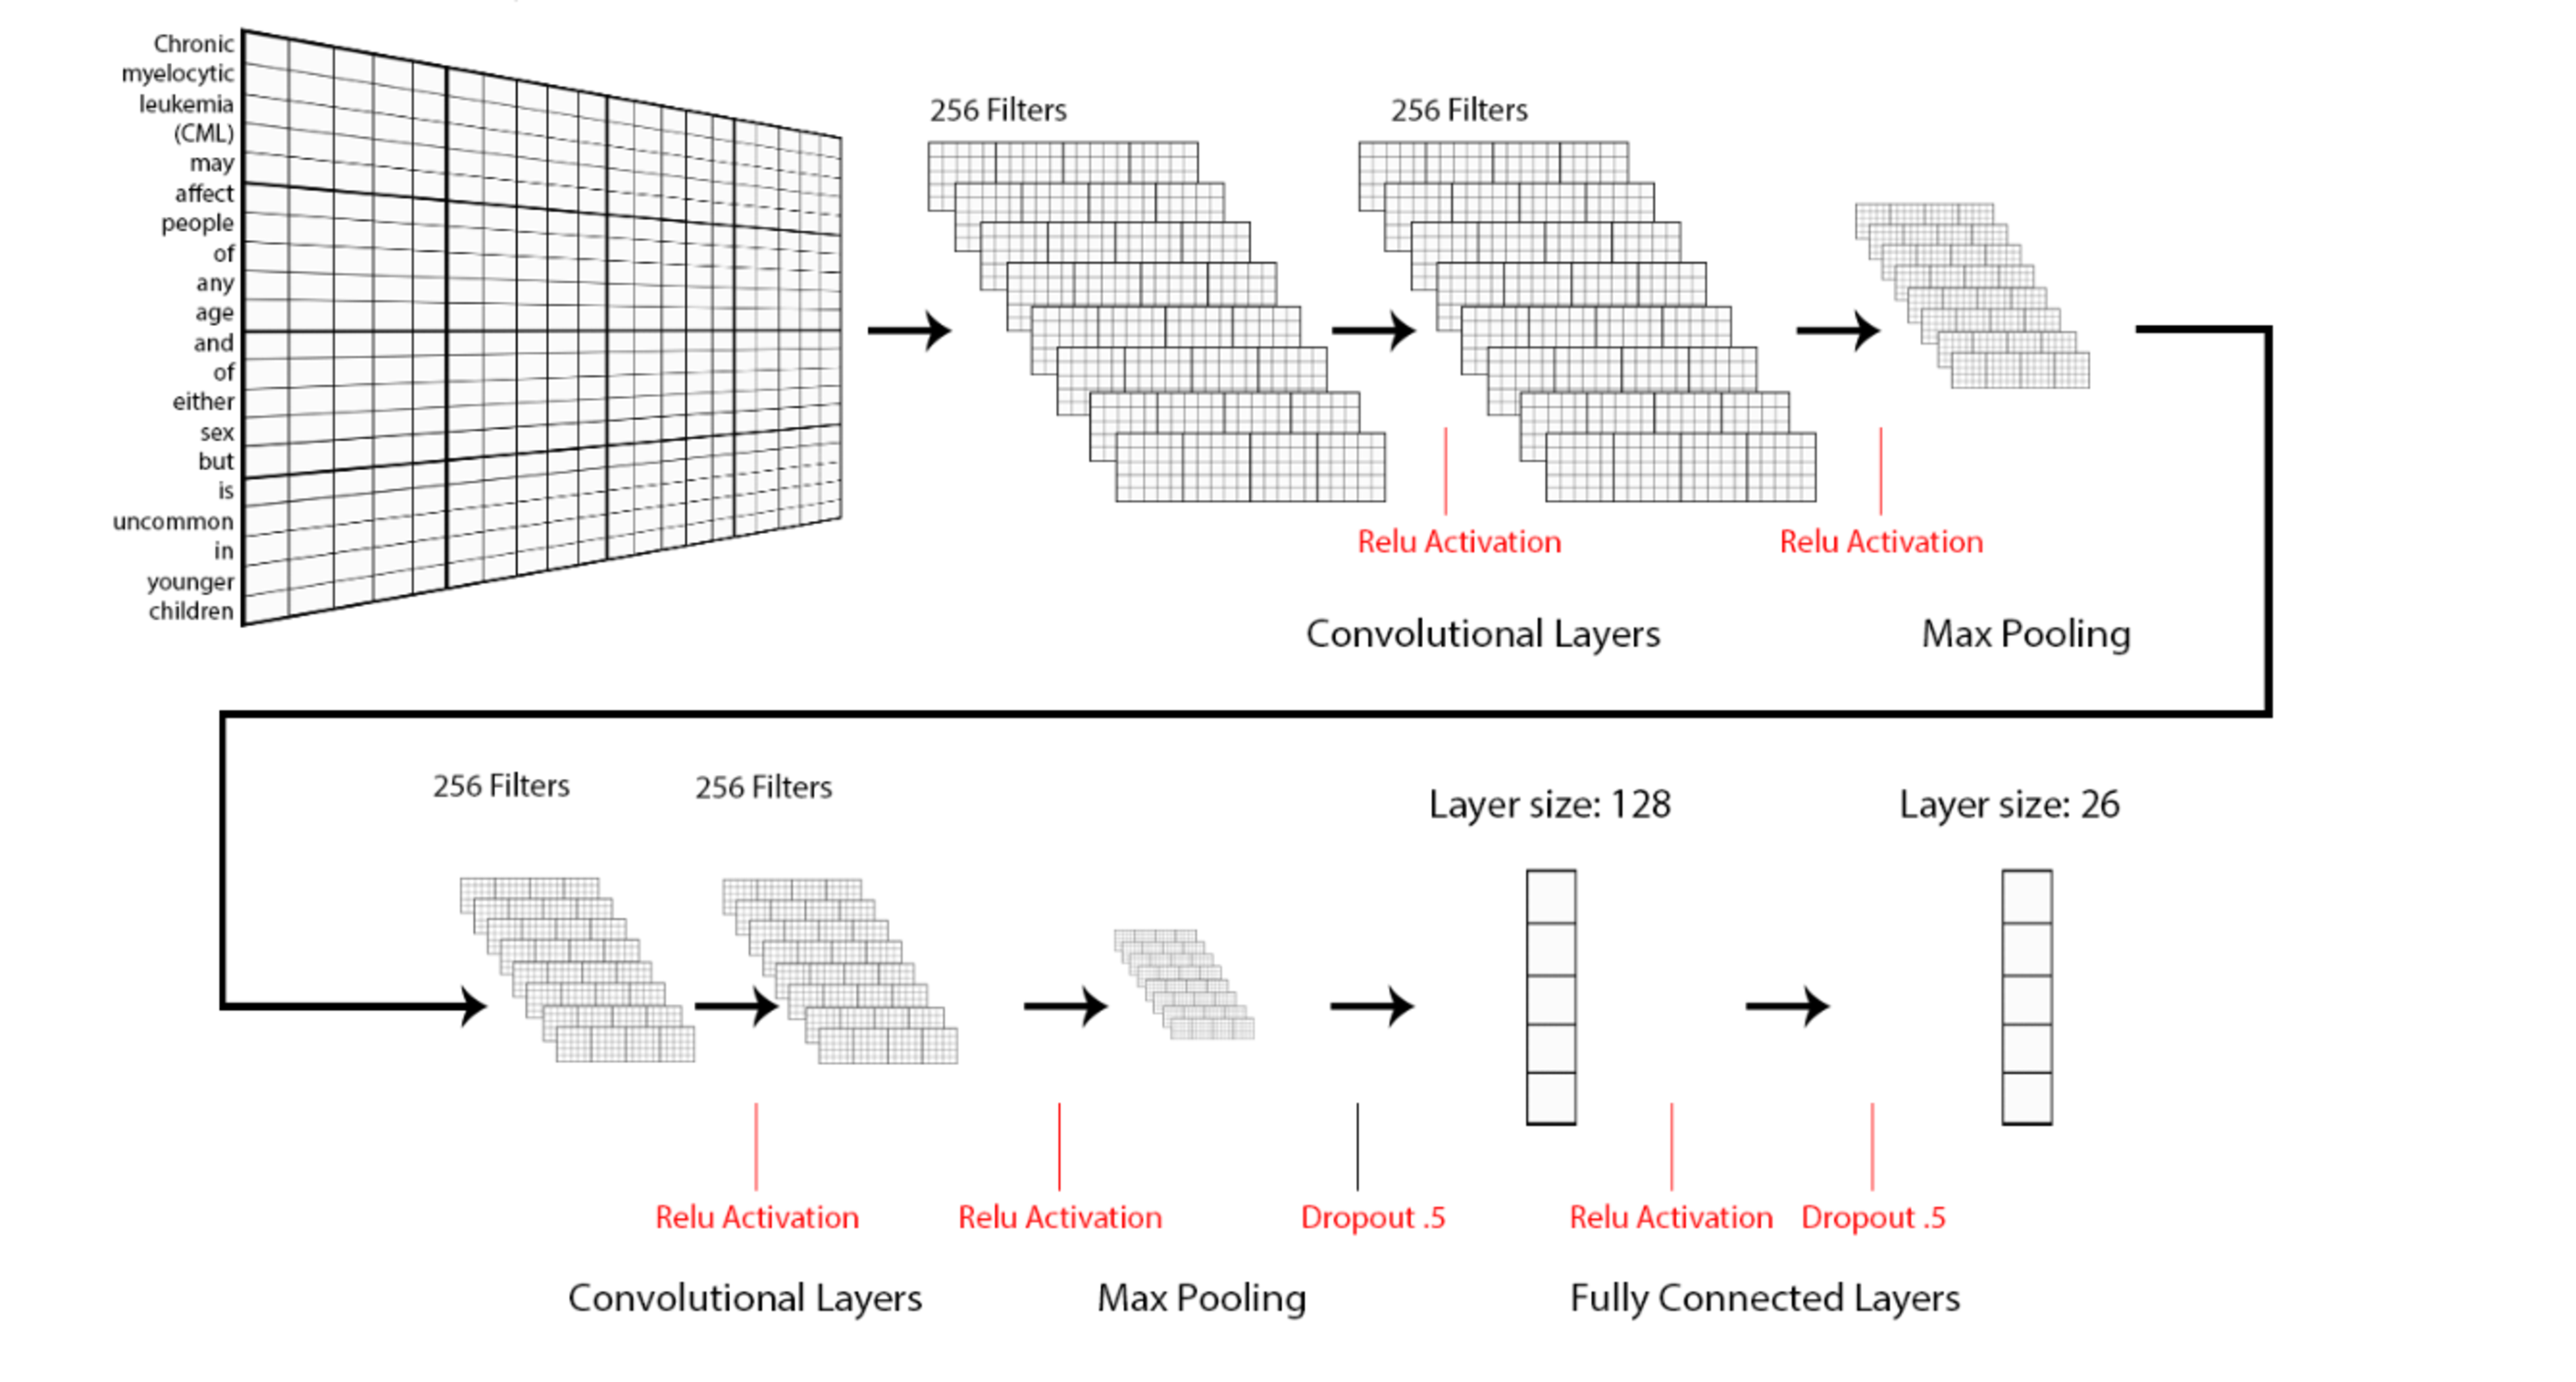
\includegraphics[width=0.5\textheight]{medicalCNN}
	\end{figure}
	\par 基于卷积神经网络的模型在结构上大体相似,区别主要在于使用的卷积层使用的层数、模型的参数和使用的池化函数不同。
	
\subsubsection{基于循环神经网络的模型}
	卷积神经网络无法捕获文本的词序信息,但是不同字母次序构成不同词,不同词序构成不同的短语或句子,不容句子词序构成文本,这都说明序列信息有很大的价值。循环神经网络正是可以将任意长度的序列表示成定长的向量的结构。循环神经网络,尤其是哪些带有们结构如LSTM和GRU的RNN结构,在捕获线性输入的统计规律方面非常有效。
	\par 最基本的循环神经网络结构如下图,网络按顺序读入序列,经过中间的RNN结构(可以为LSTM或GRU等),最终输出在第m步,产生一个定长向量来表征这个输入序列。通常我们可以将中间的RNN结构扩展为两层,一个以给出的顺序读入句子序列,另一个则以逆序读入句子序列,这样便构造了一个双向循环神经网络。Li等人在2015年证实了双向模型在句子表达上有相当好的结果。
	\begin{figure}[H]
		\centering 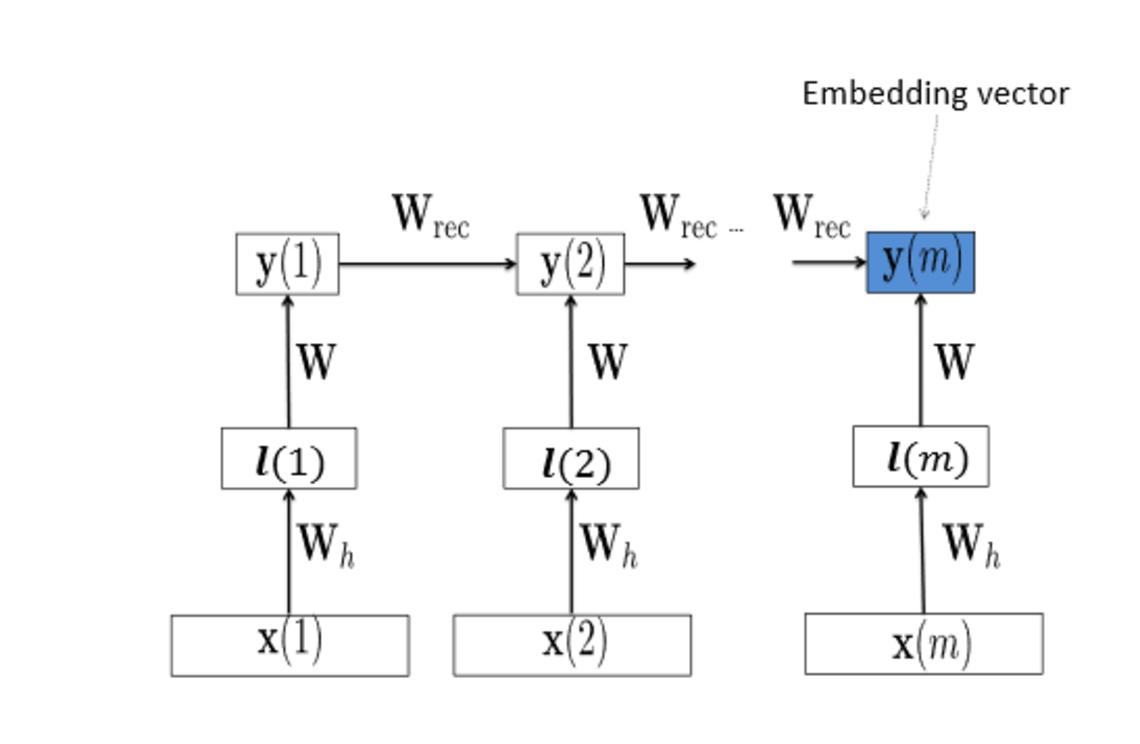
\includegraphics[width=0.5\textwidth]{BasicRNN}
	\end{figure}
	\par 当遇到文本中句子很长的情况时,结合双向结构和层次化结构很有帮助。Yang等人2016年提出了带注意力机制的层次网络模型(Hierarchical Attention Network),模型中设计了一个两层结构,分别是词级别的attention层和句子级别的attention层,每一层都是带GRU结构的双向循环神经网络,其结构如下。
	\begin{figure}[H]
		\centering 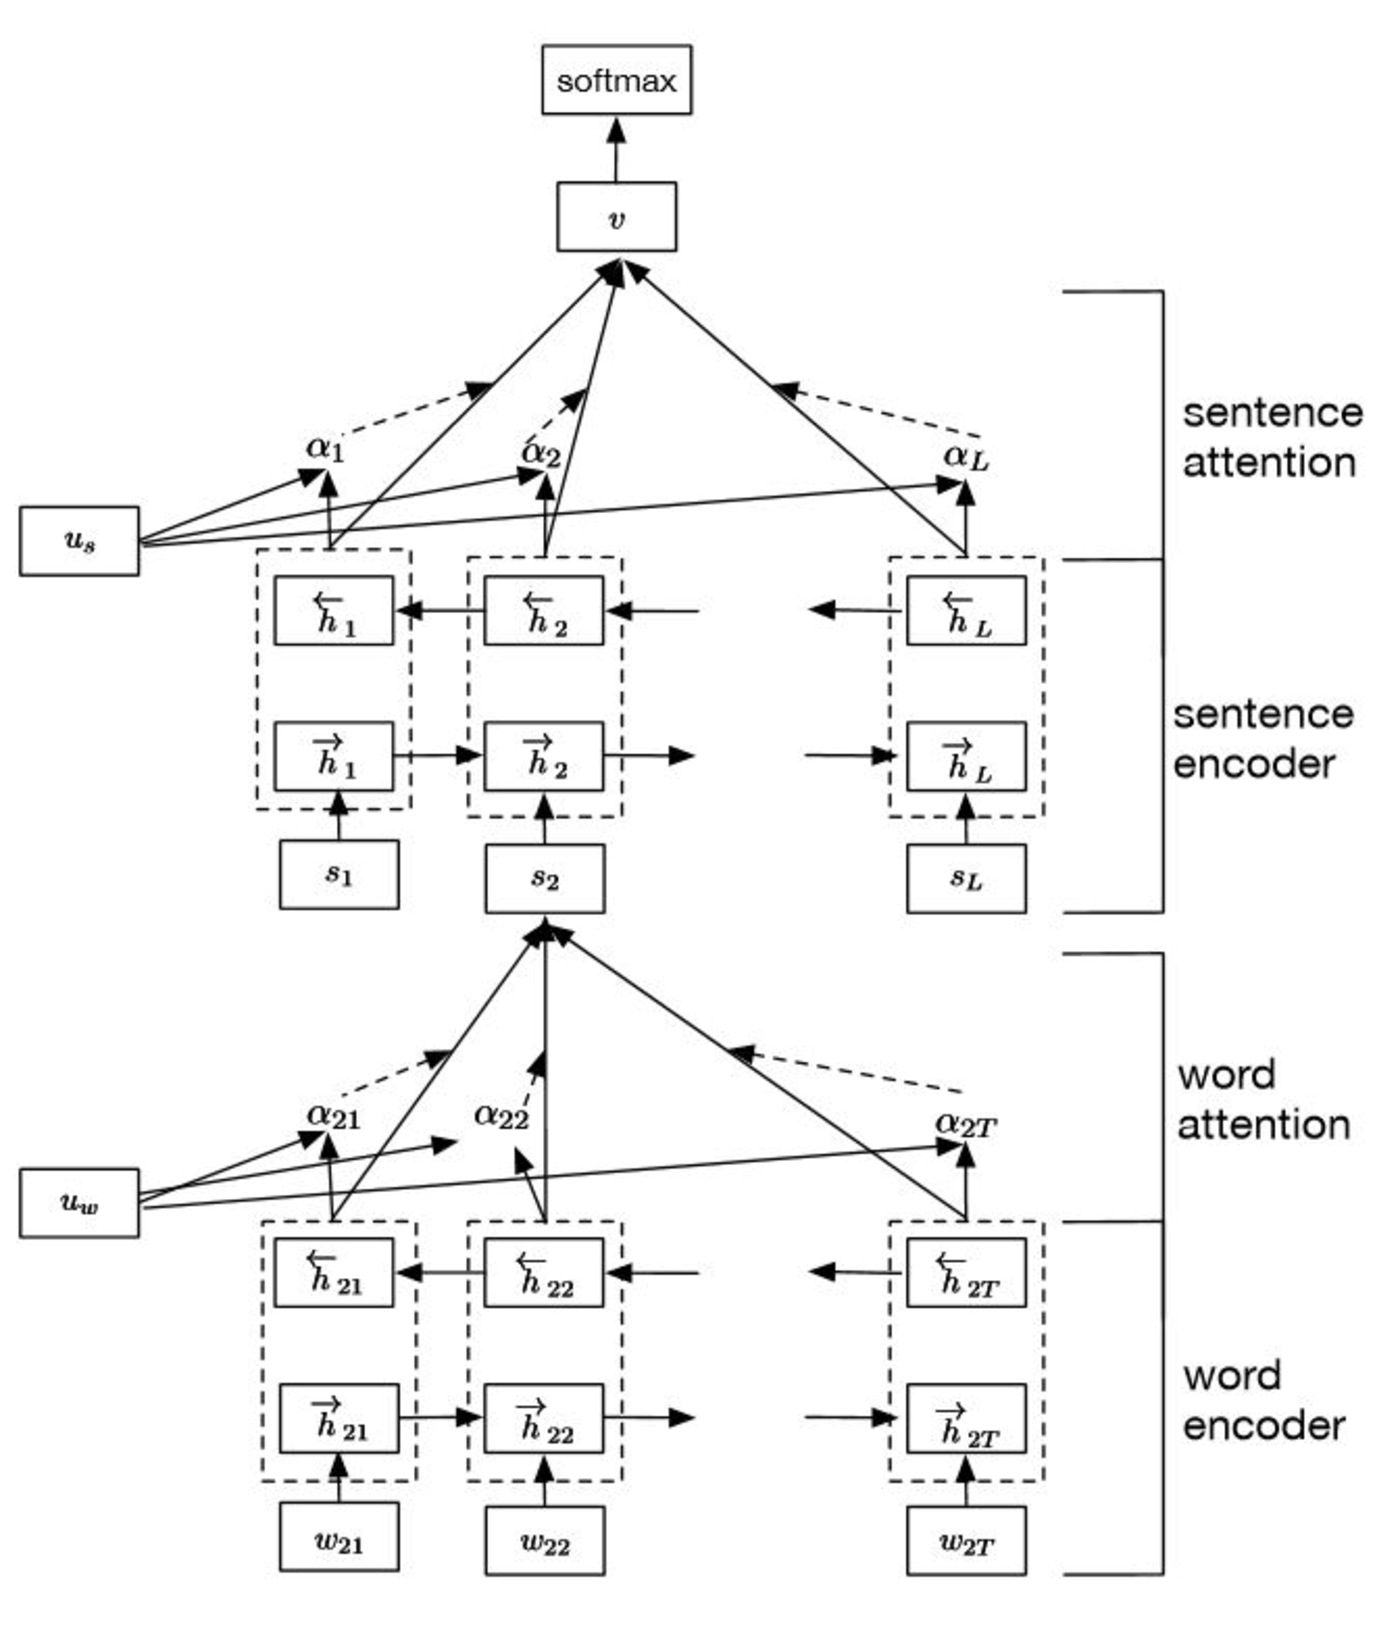
\includegraphics[width=0.5\textwidth]{AHN}
	\end{figure}
	在上述模型的第一层词级attention层,由词序列组成$w_{it} ,t\in [0,T]$组成的句子,首先把词转化成词向量,$x_{it}=W_{e}w_{it}$,然后用双向的GRU网络,可以将正向和反向的上下文信息结合起来,获得隐藏层输出。
	\begin{align*}
		x_{it}=W_{e}w_{it},t\in[1,T]\\ 
		\overrightarrow{h_{it}}=\overrightarrow{GRU}({x_{it}})\\
		\overleftarrow{h_{it}}=\overleftarrow{GRU}({x_{it}})
	\end{align*}
	对于一个给定的词语$w_{it}$,经过GRU网络后,我们获得了一种新的表示:$h_{it}=[\overrightarrow{h_{it}},\overleftarrow{h_{it}}]$$h_{it}$包含了$w_{it}$周围两个方向的信息。
	\par attention层次机制的目的是要把一个句子中,对句子的含义最重要,贡献最大的词语找出来。通过将$h_{it}$输入到一个单层的感知机中得到的结果$u_{it}$作为$h_{it}$的隐含表示。$u_{it}=tanh(W_{w}h_{it}+b_{w})$
	为了衡量单词的重要性,用$u_{it}$和一个随机初始化的上下文向量$u_{w}$的相似度来表示,然后经过softmax操作获得了一个归一化的attention权重矩阵$\alpha _{it}$,代表句子i中第t个词的权重。
	\begin{displaymath}
		\alpha _{it}=\frac{exp\left( u_{it}^{\top } u_{w}\right) }{\sum_{t}^{}{exp\left( u_{it}^\top u_{w} \right) }}
	\end{displaymath}
	有了attention权重矩阵以后,我们可以将句子向量$s_{i}=\sum_{t}{\alpha_{it}h_{it}}$看作组成这些句子的词向量的加权求和。这里的上下文向量$u_{w}$是在训练网络的过程中学习获得的。句子级别的attention层采用和词级别一样的处理方式,最终将得到的输出作为文本的向量表示,进入softmax层分类。
	\par 根据Yang等人的实验结果来看,层次化attention模型不受数据集大小的限制,不管在小数据集或者大数据集取得了最好效果,原因是循环神经网络捕捉到了序列信息,而attention结构捕捉到了文本中关键词。
	\par Plank等人在2016年提出了一个通过字符级RNN将词语转换为输入的模型,该模型通过双向RNN将一个词的字符序列转换成词向量。这种方法不仅解决了Word2Vec技术中会遇到的词表覆盖问题,而且能通过字符序列捕获词中的前缀后缀信息,提供词的歧义类有效提示。
	\par 循环神经网络结构的模型能很好地捕获序列信息,在文本分类任务中,对于对词语顺序或者句子结构敏感的应用场景下,使用循环神经网络结构有很大的帮助。
	
\subsubsection{结合卷积神经网络和循环神经网络的模型}
	文本分类任务中第三类比较常见的模型结合了卷积神经网络结构和循环神经网络结构,并辅以恰当的整体结构以提高模型整体的分类效果。结合两种结构的方式有多种,一种方式是先经过循环神经网络结构,然后再经过卷积神经网络结构的,比如,在2015年由Lai等人提出的RCNN(Recurrent Convolutional Neural Networks)模型就是一个典型的例子,RCNN模型的结构如下:
	\begin{figure}[H]
		\centering 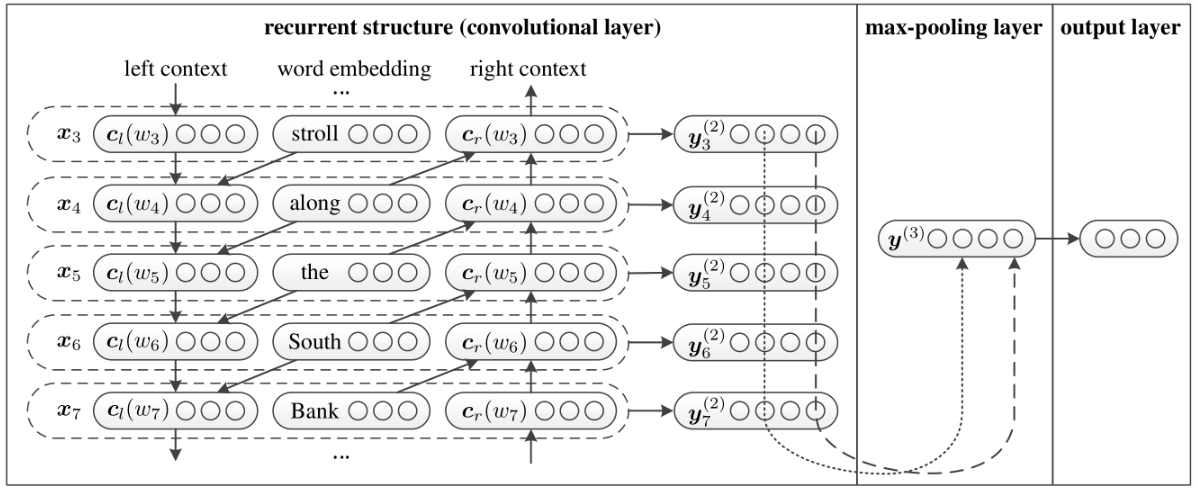
\includegraphics[width=0.5\textwidth]{RCNN}
	\end{figure}
	模型构造了一个双向循环神经网络来构造单词的上文和下文,如下式$c_l(\omega_i)$表示上文,$c_r(\omega_i)$表示下文:
	\begin{align*}
		c_l(\omega_i) = f(W^{(l)}c_l(\omega_{i-1}) + W^{(sl)}e(\omega_{i-1}) \\
		c_r(\omega_i) = f(W^{(l)}c_r(\omega_{i-1}) + W^{(sr)}e(\omega_{i-1})
	\end{align*}
	得到上下文之后用拼接方式得到单词的向量表示,$x_i = [c_l(\omega_i);e(\omega_i);c_r(\omega_i)]$,得到的词向量表示作为下一层卷积层的输入,得到潜在语义向量,然后进入池化层,即将刚刚得到的所有单词的潜语义向量中每个维度上最大的值选出组成一个新的向量,采用max-pooling可以将向量中最大的特征提取出来,从而获取到整个文本的信息。得到文本特征向量之后,进行分类。
	\par 另一种流行的方式是首先经过卷积神经网络结构,然后再经过循环神经网络结构。如Chen等人在2017年提出了一个CNN-RNN分类模型,Wang等人在2016年提出的C-LSTM模型,Liang等人2016年提出的AC-BLSTM模型等。以Chen等人提出的CNN-RNN分类模型为例,首先通过卷积神经网络结构获取文本的特征向量,之后再经过循环神经网络结构进行分类,其模型结构如下:
	\begin{figure}[H]
		\centering 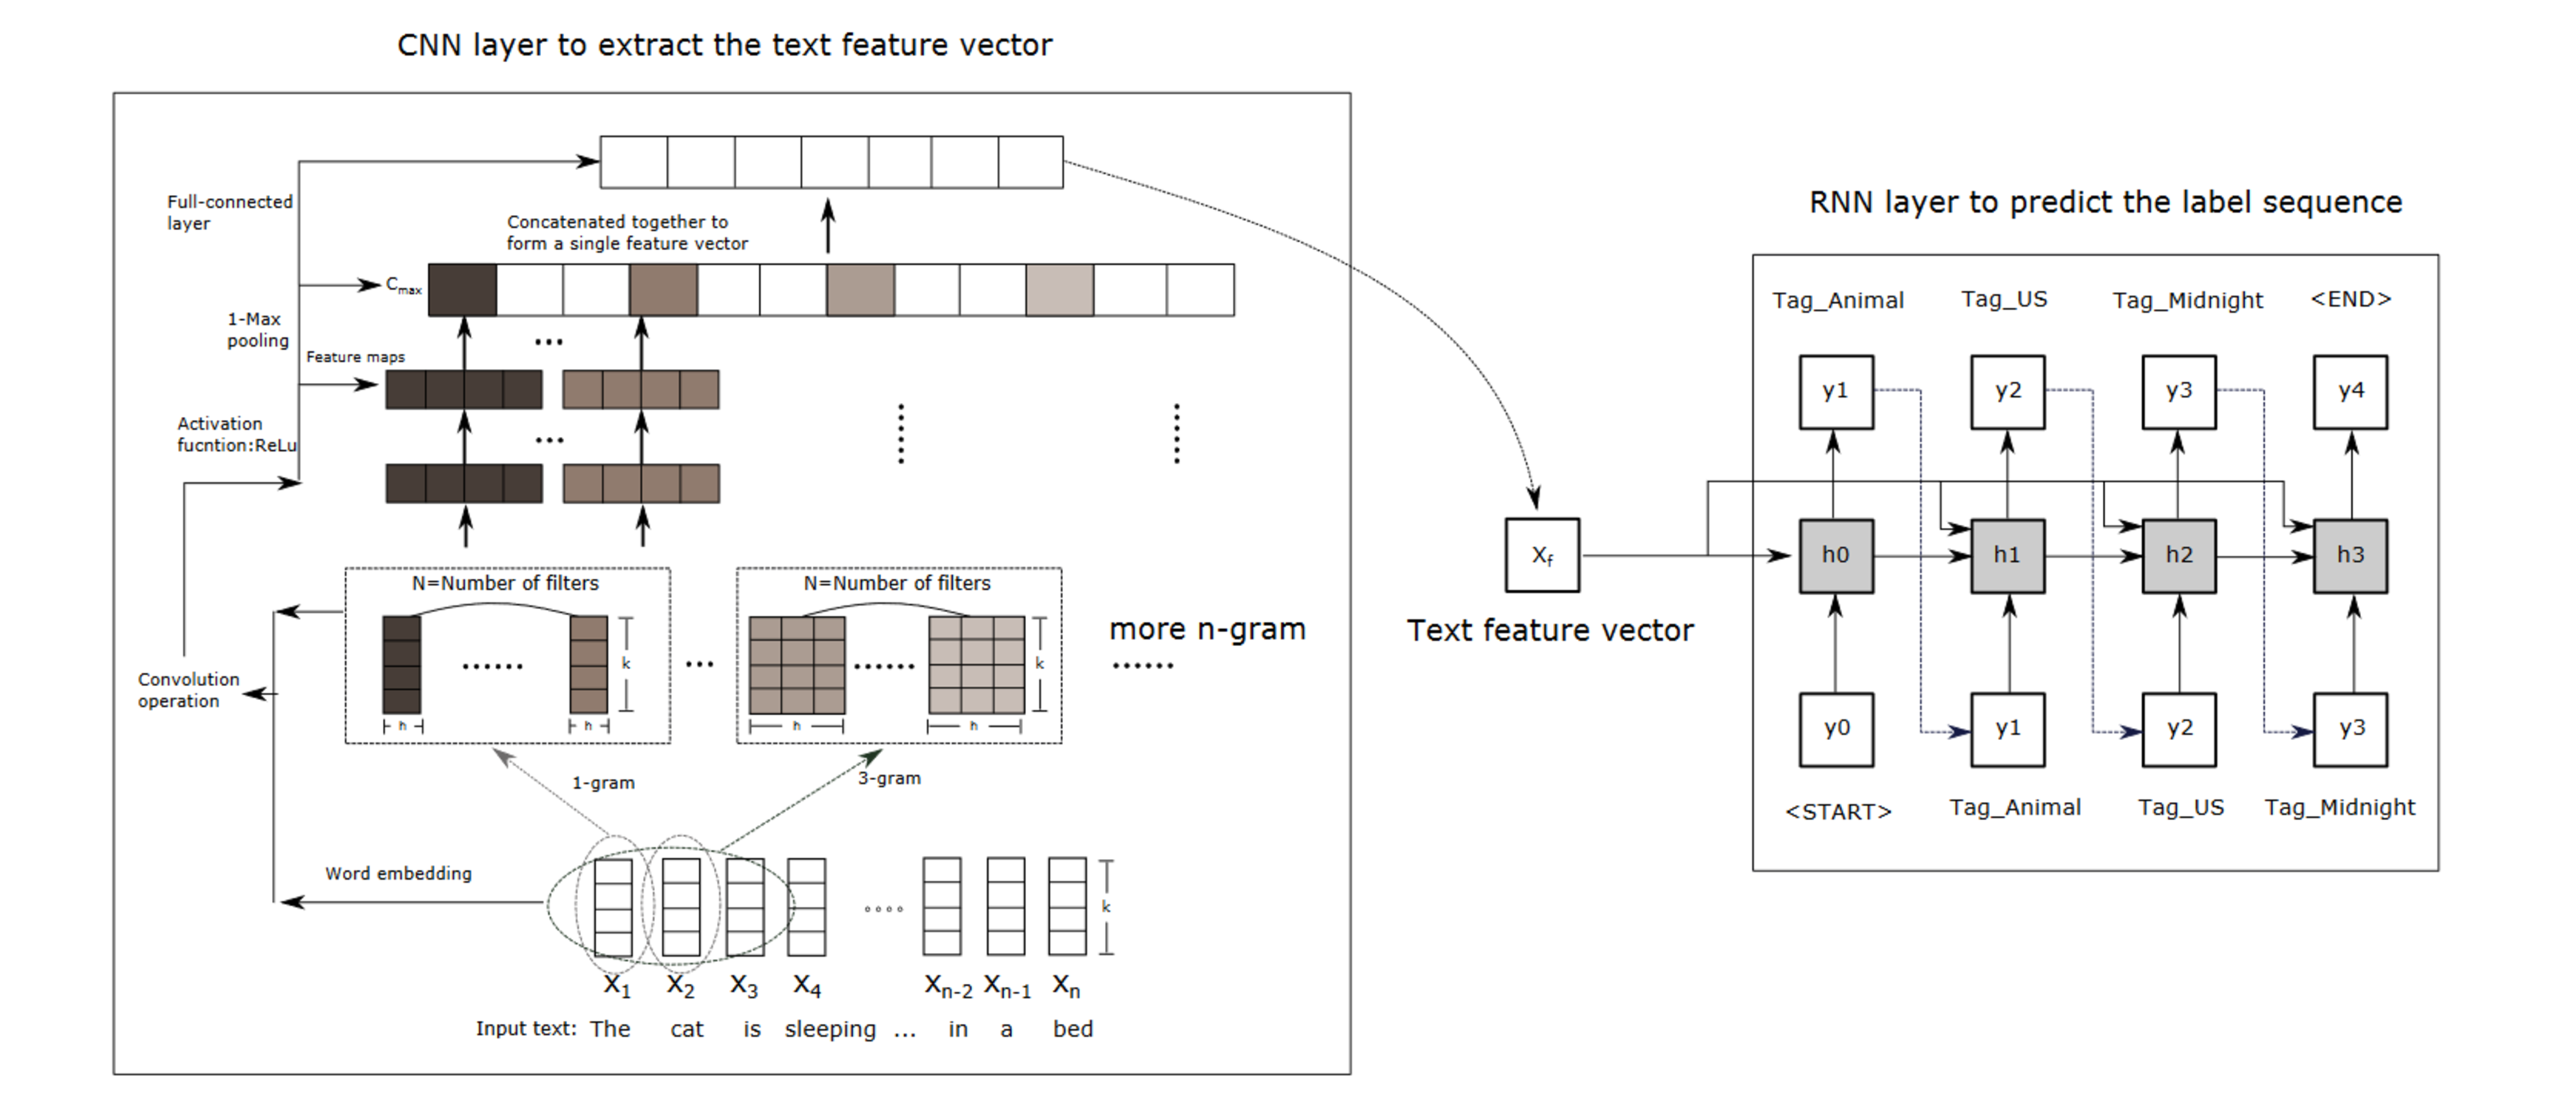
\includegraphics[width=0.7\textwidth]{CRNN}
	\end{figure}
	在该模型首先是一个具有卷积层,最大池化层和全连接层的结构,用来将文本句子生成文本特征向量,然后生成的文本特征向量作为输入序列数据进入下一个单向循环神经网络结构,得到最后的特征向量,用以分类。
	\par 除去上述两种典型的结合卷积神经网络和循环神经网络的方式,也还有采用其他方式的,比如将多个卷积神经网络结构和循环神经网络结构以不同的词序堆叠。无论哪种结合方式,利用了两种模型的优点,提升了文本分类的性能。这也提供了一种研究思路,因为每一种模型都有其鲜明的优点和无法回避的缺点,如何利用别的模型的优点来弥补自身模型的缺点,是改进模型的一种重要思路。

\section{总结}
	目前文本分类领域的研究愈发倾向于神经网络的方法,但是像朴素贝叶斯、SVM等传统机器学习分类方法凭借着其实现简单,训练速度快,效率高等优点仍然被很多地方采用。神经网络分类方法由于模型参数多,因此训练的时间和对内存要求高,但是其能够解决文本表示的稀疏性和离散性的问题,模型的分类效果也很好。当然神经网络分类模型仍有很多值得深入研究的方面,一是文本的表示,分布式表示是神经网络中的标准表示方法,也有流行的Word2Vec算法实现,是否有方法可以获得更好的分布式表示也是值得研究的问题。二是模型的结构设计和改进,如何结合各种基本模型的优点,是改进模型的一种重要思路,比如加入层次结构和attention机制都是很好的尝试。


\end{document}